%% ITEM 0 TYPE Section
\section{Pain points of existing graph-based ANNS methods}%% ITEM 1 TYPE Frame
%% ITEM 1 TYPE Frame
\begin{frame}
{Pain Points of Traditional Graph-Based ANNS}
\centering
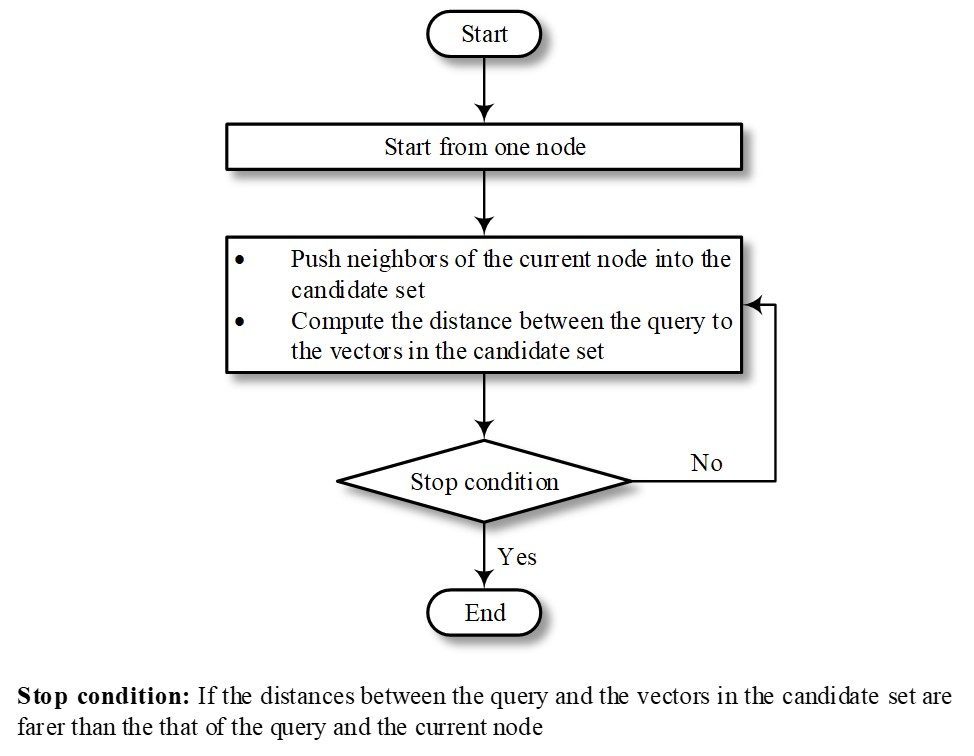
\includegraphics[width=0.8\textwidth,height=0.6\textheight,keepaspectratio]{picture/search_process.jpg}
\begin{center}
\textbf{Traditional graph-based ANNS search process} \cite{wang2021comprehensive}
\end{center}
\end{frame}%% ITEM 2 TYPE Frame
%% ITEM 2 TYPE Frame
\begin{frame}
{Key Limitations and Need for Innovation}
\begin{itemize}
\item \textbf{Distance computation dominates time cost} - accounts for most search overhead
\item \textbf{Fixed-size candidate sets} throughout search limit optimization
\item \textbf{Lack adaptive strategies} - no distinction between early exploration vs. late refinement
\item \textbf{Single-graph approaches} cannot balance speed and accuracy effectively
\item \textbf{Need multi-stage search} with different strategies for different phases
\end{itemize}
\end{frame}%% ITEM 3 TYPE Section
%% ITEM 3 TYPE Section
\section{CSPG approach with partitioning algorithm}%% ITEM 4 TYPE Section
%% ITEM 4 TYPE Section
\section{CSPG Approach with Partitioning Algorithm}%% ITEM 5 TYPE Frame
%% ITEM 5 TYPE Frame
\begin{frame}
{Core Idea: Partitioning for Adaptive Search}
\centering
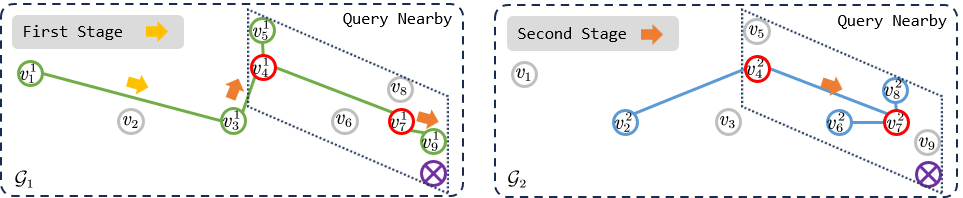
\includegraphics[width=0.8\textwidth,height=0.6\textheight,keepaspectratio]{picture/method.png}

\vspace{5mm}
\begin{itemize}
    \item \textbf{Random partitioning} of dataset into multiple groups
    \item \textbf{Shared routing vectors} (red) connect different partitions
    \item Each partition has its own \textbf{sparser proximity graph}
    \item Enables: \textbf{Large steps when far} (speed) + \textbf{Small steps when close} (accuracy)
\end{itemize}
\end{frame}%% ITEM 6 TYPE Frame
%% ITEM 6 TYPE Frame
\begin{frame}
{Two-Stage Search Process}
\centering
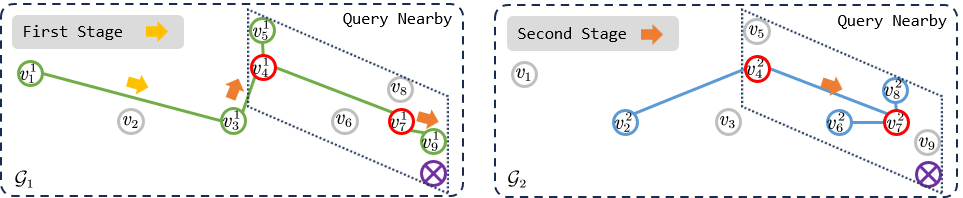
\includegraphics[width=0.7\textwidth,height=0.5\textheight,keepaspectratio]{picture/method.png}

\vspace{3mm}
\begin{minipage}{0.9\textwidth}
\begin{block}{\textbf{Stage 1: Fast Approaching (Yellow arrows)}}
\begin{itemize}
    \item Greedy beam search within \textbf{single partition}
    \item Smaller candidate set size ($ef_1$) for speed
    \item Quickly narrows search to query vicinity
\end{itemize}
\end{block}

\begin{block}{\textbf{Stage 2: Precise Search (Orange arrows)}}
\begin{itemize}
    \item Cross-partition expansion using routing vectors
    \item Larger candidate set ($ef_2 > ef_1$) for accuracy
    \item When encountering routing vector: add \textbf{all instances} from all partitions
\end{itemize}
\end{block}
\end{minipage}
\end{frame}%% ITEM 7 TYPE Frame
%% ITEM 7 TYPE Frame
\begin{frame}
{Key Benefits and Summary}
\centering
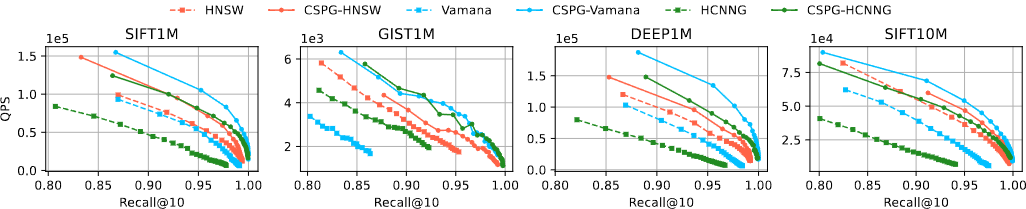
\includegraphics[width=0.6\textwidth,height=0.4\textheight,keepaspectratio]{picture/perf.png}

\vspace{3mm}
\begin{minipage}{0.9\textwidth}
\begin{itemize}
    \item \textbf{Adaptive search}: Large steps when far, small steps when close
    \item \textbf{Efficient cross-partition exploration} via routing vectors
    \item \textbf{Memory efficient}: Each partition has smaller, sparser graph
    \item \textbf{High recall with low latency} compared to baseline methods
\end{itemize}
\end{minipage}

\vspace{5mm}
\begin{block}{\textbf{Summary}}
CSPG partitions dataset randomly, creates smaller proximity graphs per partition, and uses two-stage search with routing vectors for efficient cross-partition exploration.
\end{block}
\end{frame}%% ITEM 8 TYPE Section
%% ITEM 8 TYPE Section
\section{Two-stage search method and contributions}%% ITEM 9 TYPE Frame
%% ITEM 9 TYPE Frame
\begin{frame}
\begin{center}
\Large \textbf{CSPG: Two-Stage Search Method}
\end{center}

\vspace{0.3cm}

\textbf{Key Innovation: Two-Stage Search Strategy}

\begin{itemize}
    \item \textbf{Stage 1: Fast Approaching}
    \begin{itemize}
        \item Uses only \textbf{one proximity graph} for initial search
        \item Goal: Quickly get close to query point
        \item Small candidate set size: \textbf{ef₁}
    \end{itemize}
    
    \item \textbf{Stage 2: Precise Search}
    \begin{itemize}
        \item Considers \textbf{all groups} for refinement
        \item Goal: Achieve high accuracy
        \item Larger candidate set size: \textbf{ef₂} (ef₁ < ef₂)
    \end{itemize}
    
    \item \textbf{Different from traditional beam search} which uses same ef for all stages
\end{itemize}

\vspace{0.3cm}

\textbf{Why This Works:}
\begin{itemize}
    \item Stage 1 reduces search space efficiently
    \item Stage 2 ensures high recall with minimal overhead
    \item Adaptive candidate sizes optimize speed-accuracy tradeoff
\end{itemize}
\end{frame}%% ITEM 10 TYPE Frame
%% ITEM 10 TYPE Frame
\begin{frame}
\begin{center}
\Large \textbf{Experimental Results \& Contributions}
\end{center}

\vspace{0.3cm}

\textbf{Benchmark Datasets:}
\begin{itemize}
    \item SIFT1M: 1M 128-dimensional SIFT descriptors
    \item GIST1M: 1M 960-dimensional GIST descriptors
    \item DEEP1M: 1M 96-dimensional deep features
    \item SIFT10M: 10M 128-dimensional SIFT descriptors
\end{itemize}

\vspace{0.3cm}

\textbf{Key Performance Improvements:}

\begin{itemize}
    \item \textbf{Higher QPS (Queries Per Second)} than traditional proximity graphs
    \item \textbf{Higher Recall@10} across all benchmark datasets
    \item Maintains competitive performance on larger datasets (SIFT10M)
    \item Outperforms state-of-the-art methods in speed-accuracy tradeoff
\end{itemize}

\vspace{0.3cm}

\textbf{Main Contributions:}
\begin{itemize}
    \item Novel two-stage search with adaptive candidate sizes
    \item Efficient partitioning strategy for graph construction
    \item Demonstrated superior performance on standard benchmarks
    \item Open-source implementation available for reproducibility
\end{itemize}
\end{frame}%% ITEM 11 TYPE Frame
%% ITEM 11 TYPE Frame
\begin{frame}
\begin{center}
\Large \textbf{Summary \& Conclusion}
\end{center}

\vspace{0.5cm}

\textbf{CSPG's Key Innovations:}

\begin{itemize}
    \item \textbf{Two-stage search}: Fast approaching + precise refinement
    \item \textbf{Adaptive candidate sizes}: ef₁ < ef₂ for optimal tradeoff
    \item \textbf{Different from traditional beam search} with fixed ef
\end{itemize}

\vspace{0.5cm}

\textbf{Proven Results:}

\begin{itemize}
    \item \textbf{Higher QPS} and \textbf{higher Recall@10}
    \item Validated on SIFT1M, GIST1M, DEEP1M, SIFT10M
    \item Superior speed-accuracy tradeoff
\end{itemize}

\vspace{0.5cm}

\begin{center}
\large \textbf{CSPG advances ANN search with smarter, adaptive algorithms}
\end{center}
\end{frame}
%% ITEM 12 TYPE Frame
\begin{frame}
\begin{itemize}
\item Item 1
\end{itemize}
\end{frame}